\documentclass{beamer} 
%\documentclass[handout]{beamer} 

% Michael Maier, 2016.
% CC-0

\usepackage[utf8]{inputenc}
\usepackage[ngerman]{babel}

\title{Rollstuhlrouting mit OpenStreetMap}
\author{Michael Maier \textless Michael.Maier@student.tugraz.at\textgreater} 
\date{17. November 2016} 

\usetheme{Antibes}

\newcommand{\boldm}[1] {\mathversion{bold}#1\mathversion{normal}}

\hypersetup{colorlinks=true,urlcolor=blue,linkcolor=white}

%\usebackgroundtemplatei{
%
\includegraphics[width=\paperwidth,
%height=0.8\paperheight]{mag_map.png}
%}

\begin{document}

%\maketitle

\begin{frame} 


\begin{figure}
  \centering
  
\includegraphics[width=.4\textwidth]{mag_map.png}
\end{figure}

\begin{center}
\Large{\emph{Rollstuhlrouting mit OpenStreetMap}}
\end{center}

\end{frame}


\section{Einleitung}

\begin{frame}{Vorstellung}

  \begin{itemize}
    \item Michael Maier \textless \href{mailto:Michael.Maier@mailbox.org}{Michael.Maier@mailbox.org}\textgreater
    \item Student an der TU Graz (Telematik)
\vspace{0.3cm}
    \item Linux-User (Debian/grml) seit 2004
    \item Organisiere Grazer Linuxtage seit 2011 mit
    \item OpenStreetMap als Hobby seit Juli 2010
    \item Leite den Grazer OSM-Stammtisch seit Mai 2011
\vspace{0.3cm}
    \item Vorträge und Workshops zum Thema OSM seit 2012
    \item Freiberuflich OSM-Aufträge und Consulting
    \begin{itemize}
      \item OSM-username: \emph{\href{http://www.openstreetmap.org/user/species}{species}}
      \item Github-Account: \emph{\href{https://github.com/species}{species}}
      \item Twitter-Account: \emph{\href{https://twitter.com/osmgraz}{@osmgraz}}
    \end{itemize}
  \end{itemize}
\end{frame}

\section{OpenStreetMap}
\begin{frame}{OpenStreetMap}

\begin{itemize}
  \item OpenStreetMap (OSM) ist eine freie Weltkarte nach dem Wiki-Prinzip "`Wikipedia der Karten"'
    \begin{itemize}
      \item \emph{Eigentlich eine Geo-Datenbank}
    \end{itemize}

          \pause
            \item Entsteht aus der Arbeit von \textgreater 3\,M Hobbykartografen "`\emph{Mapper}"'
          \end{itemize}

           \begin{center}
              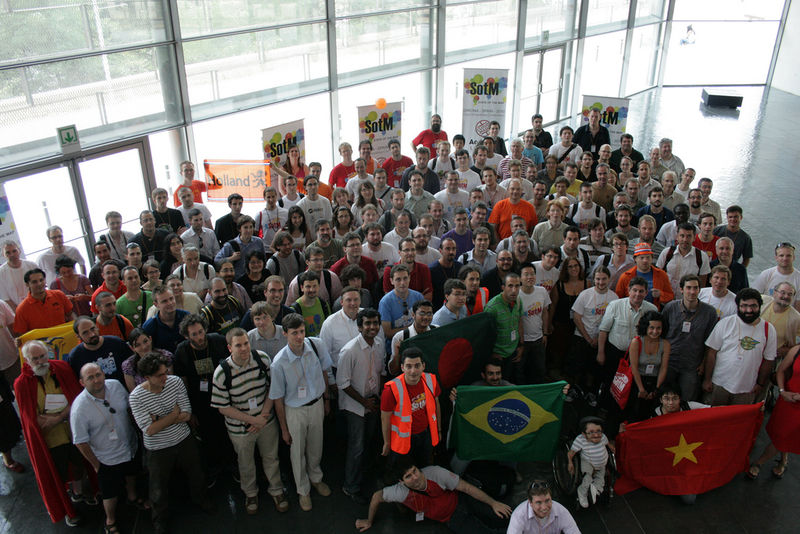
\includegraphics[width=4.5cm]{sotm.jpg}
               \end{center}

\end{frame}


\subsection{Wie funktioniert OpenStreetMap?}
% * Technogie, Datenmodell, Lizenz

\begin{frame}{Woher kommen unsere Daten?}

\begin{itemize}
  \item Ursprünglich: GPS-Tracks
  \item Freiwillige tragen ihr Wissen bei: Jeder weiß viel über seine Umgebung:
  \begin{itemize}
    \item Hausnummern, Straßennamen,
    \item Restaurants, Bars, POIs, \dots
  \end{itemize}
  \pause
  \item Bei Mapping-Parties werden \\ gezielt Gebiete verbessert
\end{itemize}

  \vspace{0.4cm}
 99\% Handarbeit!

  \vspace*{-2.9cm}
 \hfill 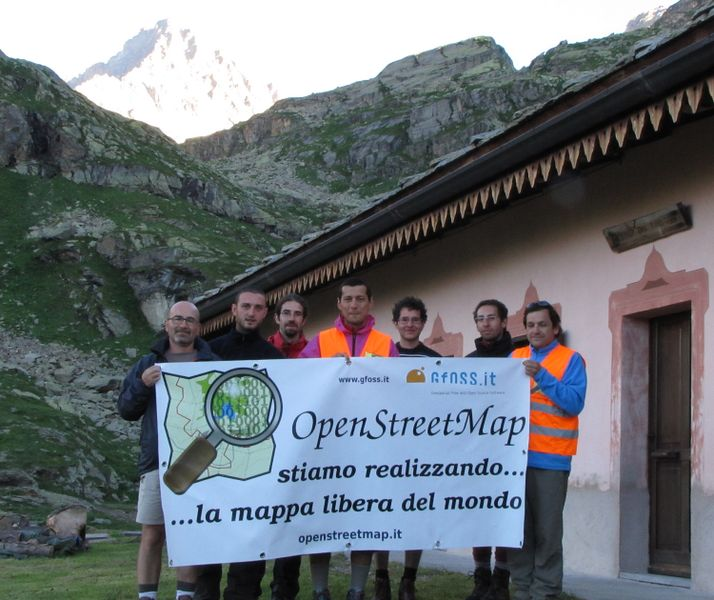
\includegraphics[width=4.2cm]{alps_mp.jpg}


  \pause
\begin{itemize}
  \item Hin und wieder Importe aus Open Government Data
  \begin{itemize}
    \item USA, TIGER Data (2008)
    \item Dänemark, Hausnummern (laufend synchronisiert)
    \item Wien, Baumkataster
  \end{itemize}
\end{itemize}

\end{frame}

\subsection{Lizenz}

\begin{frame}{Lizenz}

  Die Daten stehen unter der \emph{Open Database Licence} - Entspricht etwa Creative Commons - Attribution - Sharealike für Daten.

 \begin{center}
 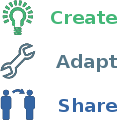
\includegraphics[width=1cm]{ODbL.png}
 \hspace{2cm}
 
\includegraphics[width=1.5cm]{cc-by-sa.pdf}
 \end{center}

\pause

\vspace*{-0.3cm}

\begin{itemize}
  \item Jeder darf die Daten, auch kommerziell verwenden, jedoch:
  \begin{itemize}
    \item Attribution "`OpenStreetMap \& Contributors, ODbL"' angeben!
    \item Share-Alike: Wer die Daten verändert, muss sie unter derselben Lizenz veröffentlichen!
    \item Diese "`virale Lizenz"' stellt sicher, dass Verbesserungen nicht in den Silos von Konzernen verschwinden, sondern der Allgemeinheit weiter zur Verfügung stehen
  \end{itemize}

\end{itemize}


\pause
Die Web-Karten auf \href{http://osm.org}{openstreetmap.org} sind CC-BY-SA.
\begin{itemize}
  \item Beachte Tile Usage Policy!
\end{itemize}

\end{frame}

\subsection{Versionierung}

\begin{frame}{Versionierung}

Der komplette Datenbestand steht unter Versionskontrolle.
\begin{itemize}
  \item Auszüge können für beliebige Zeitpunkte erstellt werden
  \item Spiegel-DB mit inkrementellen diffs minütlich aktualisierbar
  \item DB sicher gegen Korrumption durch parallele Edits durch Verwendung von Changesets
  \begin{itemize}
    \item Pro Tag werden $\sim$21.000 Changesets submitted
  \end{itemize}
  \item Für jedes Objekt ist seine gesamte Historie abrufbar
\end{itemize}

% \vspace*{-3cm}
 \hfill 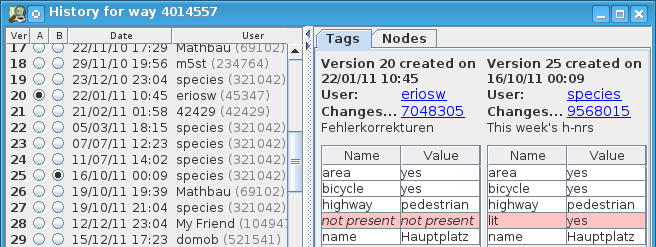
\includegraphics[width=8cm]{history.png}


\end{frame}


\section{Projekt wheelroute.at}

\begin{frame}{Projekt Wheelroute.at - Ziele}


    \begin{itemize}
       \item Barrierefreiheit im Innenstadtbereich überprüfen

         \pause

      \vspace{1cm}

      \item Rückmeldung an die Stadt Graz, wo Prioritäten für Verbesserungen liegen
    \end{itemize}

Gesponsert vom Verein ``In!tiativ für Menschen mit Behinderung''

\end{frame}

\begin{frame}{Erfasste Gebiete}

  \begin{columns}[c]
    \begin{column}[T]{.6\textwidth}
      \begin{center}
      \vspace{-1cm}
      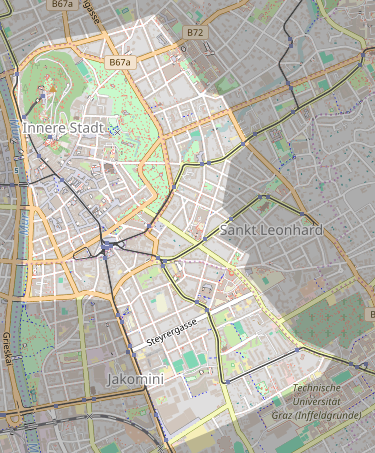
\includegraphics[width=6cm]{gebiet.png}
      \end{center}
    \end{column}
    \begin{column}[T]{.4\textwidth}
      \begin{itemize}
            \item 3,2 km$^2$
            \item Innere Stadt bis Karl-Franzens-Uni
    \item       Karl-Franzens-Uni bis TU (Inffeld)
  \item       Jakominiplatz bis Messe
      \vspace{1cm}
  \item       Nach demselben Schema wurde vor 3~Jahren die Stadt Gleisdorf erfasst.
    \end{itemize}
    \end{column}
  \end{columns}

\end{frame}

\begin{frame}{Erfassung}
Was wurde erfasst?

    \begin{itemize}
      \item Bordsteinkanten-Höhen
      \item Steigungen, Querneigungen
      \item Breiten
      \item Oberfläche
      \item Fußgängerampeln und taktile Bodenmarkierungen
    \end{itemize}


Wie wurde erfasst?
    \begin{itemize}
      \item Rollmaß für Breiten und Kantenhöhen
      \item Digitale Wasserwaage für Steigungen und Querneigungen
      \item Papier \& Bleistift
      \item Fotos bei kritischen Stellen
    \end{itemize}

\end{frame}


\subsection{Ergebnisse}

\subsection{Routing}

\begin{frame}{}

  \begin{columns}[c]
    \begin{column}[T]{.6\textwidth}
      \begin{center}
      \vspace{-1cm}
      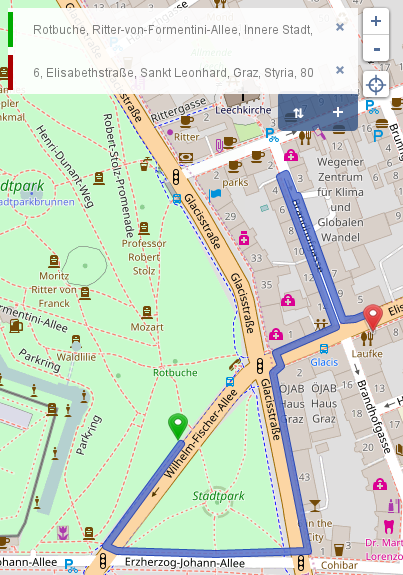
\includegraphics[width=5.5cm]{routing1_normal.png}
      \end{center}
    \end{column}
    \begin{column}[T]{.4\textwidth}
      \begin{itemize}
      \vspace{1cm}
        \item Routingservice im Beta-Stadium (\href{http://mm.linuxtage.at/osm/routing/wheelchair-normal/?z=17\&center=47.072643\%2C15.452845\&loc=47.073045\%2C15.446059\&loc=47.073841\%2C15.448145\&hl=en\&ly=\&alt=\&df=\&srv=}{Link}) auf wheelroute.at
              \pause
      \vspace{1cm}
            \item 3 Profile:
              \begin{itemize}
                \item Hand-Rolli
                \item E-Rolli
                \item Sportliche Fahrer
          \end{itemize}
        \end{itemize}

    \end{column}
  \end{columns}

\end{frame}

\subsection{Hinderniss-Karte}

\begin{frame}{}

  \begin{columns}[c]

    \begin{column}[T]{.6\textwidth}
      \begin{center}
      \vspace{-0.3cm}
      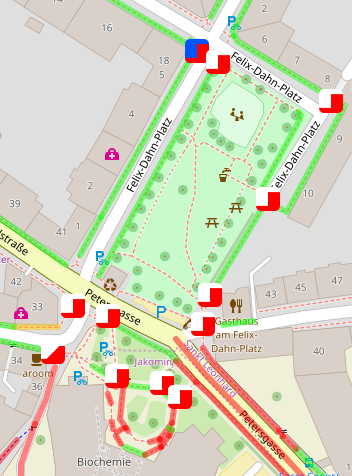
\includegraphics[width=5.5cm]{hindernisse.png}
      \end{center}

    \end{column}
    \begin{column}[T]{.4\textwidth}

      \begin{itemize}
      \vspace{1cm}
          \item Farbdarstellung mit klickbaren Elementen (\href{http://species.github.io/wheelchair-obstacles/normal.html\#18/47.06588/15.45369}{Link})

      \vspace{1cm}

            \item 3 Verschiedene Karten:

              \begin{itemize}
                \item Hand-Rolli
                \item E-Rolli
                \item Sportliche Fahrer
              \end{itemize}
        \end{itemize}

    \end{column}
  \end{columns}

\end{frame}

\begin{frame}{Beispiel für Linked Open Data: Foto-Einbindung in OSM}

  \begin{columns}[c]
    \begin{column}[T]{.6\textwidth}

      \begin{center}
      \vspace{-1cm}
      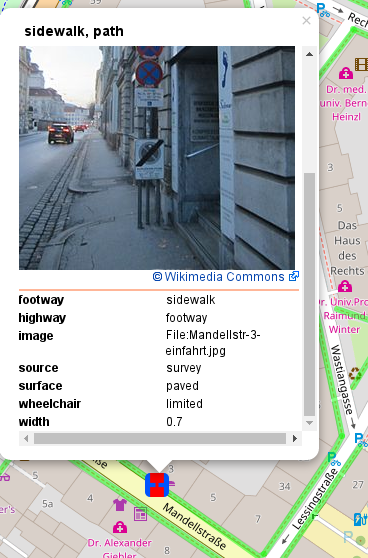
\includegraphics[width=5.5cm]{Fotos-screenie.png}
      \end{center}

    \end{column}
    \begin{column}[T]{.4\textwidth}

      \begin{itemize}
        \item Fotos wurden auf Wikimedia Commons gestellt.
        \vspace{0.5cm}
        \item Bild im OSM-Tag verlinkt via image=File:\$Bildname 
        \vspace{0.5cm}
        \item Webseite lädt Bilder (blaues Icon) dynamisch nach
        \end{itemize}

    \end{column}
  \end{columns}

\end{frame}

\begin{frame}{Statistik}

  Was haben wir gefunden?

      \begin{itemize}
        \item 137 nicht abgesenkte Gehsteigkanten
        \item 17,2 km an Wegen mit Steigungen $>$ 3\%
        \item 3,6 km an Wegen mit Querneigung $>$ 3\%
        \item 65 (teilweise) defekte Ampeln
      \end{itemize}
        
\end{frame}

\section{Ende}

\begin{frame}{Vielen Dank für die Aufmerksamkeit!}

  Folien zum Open Data Meetup am 17.11.2016, Wien
\vspace{1cm}

Erstellt mittels \LaTeX Beamer, Quelltext: \href{https://github.com/species/vortrag-osm-opendatameetup16}{Github/species/vortrag-osm-opendatameetup16}.
\vspace{1cm}

\href{mailto:Michael.Maier@student.tugraz.at}{Michael Maier}, OSM-User: species

Twitter: \href{https://twitter.com/osmgraz}{@osmgraz}
\vspace{1cm}

Folien-Quelltext unter: 
\includegraphics[width=1cm]{cc-zero.pdf}. 

\end{frame}

\end{document}
